%++++++++++++++++++++++++++++++++++++++++
% Don't modify this section unless you know what you're doing!
\documentclass[letterpaper,12pt]{article}
\usepackage{graphicx}
\usepackage{subfig}
\usepackage{tabularx} % extra features for tabular environment
\usepackage{amsmath}  % improve math presentation
\usepackage{float}
\usepackage{graphicx} % takes care of graphic including machinery
\usepackage[margin=1in,letterpaper]{geometry} % decreases margins
\usepackage{cite} % takes care of citations
\usepackage[final]{hyperref} % adds hyper links inside the generated pdf file
\hypersetup{
	colorlinks=true,       % false: boxed links; true: colored links
	linkcolor=blue,        % color of internal links
	citecolor=blue,        % color of links to bibliography
	filecolor=magenta,     % color of file links
	urlcolor=blue         
}
%++++++++++++++++++++++++++++++++++++++++


\begin{document}

\title{End Term}
\author{Aman Bagla}
\date{}
\maketitle

\section{Problem Statement}
Report to the government of "East Sound Central" region a predictive model of the total electricity used for heating (quantitative response) and identify main predictors as well.

\section{Cleaning and Pre-processing of Data}
\begin{itemize}
\item Deleted all the columns including Final Weights and Imputation information as they doesn't provide any significant information for response variable.
\item All the columns with only one unique values were deleted.
\item All the columns having categorical values converted to factors as per there respective levels using 'as.factor' command. Missing values of these columns assigned to level 'NA'.
\item Deleted all numerical predictor columns with more than 50 NA's.
\item All the incomplete observation deleted i.e. 65 observations deleted out of 393.
\item Dummy variables introduced for all categorical predictors as per there respective levels.
\item Deleted all dummy variables columns corresponding to 'NA' values of their corresponding predictor.
\end{itemize}

\section{Exploratory Data Analysis}
Exploratory data analysis performed using 'skim' command from package 'skimr'. Which shows histogram of the predictors and response.
\newline

\setlength{\parindent}{0em}
From histograms of all numerical predictors it was found that the data is highly skewed and hence a logarithmic transformation is necessary. Also, lots of observation of response and several numerical predictors were zero and logarithmic transformation was not possible hence 1 was added to all the numerical predictors and then the logarithmic transformation was performed. 
\begin{figure}[H]%
    \centering
    \subfloat{{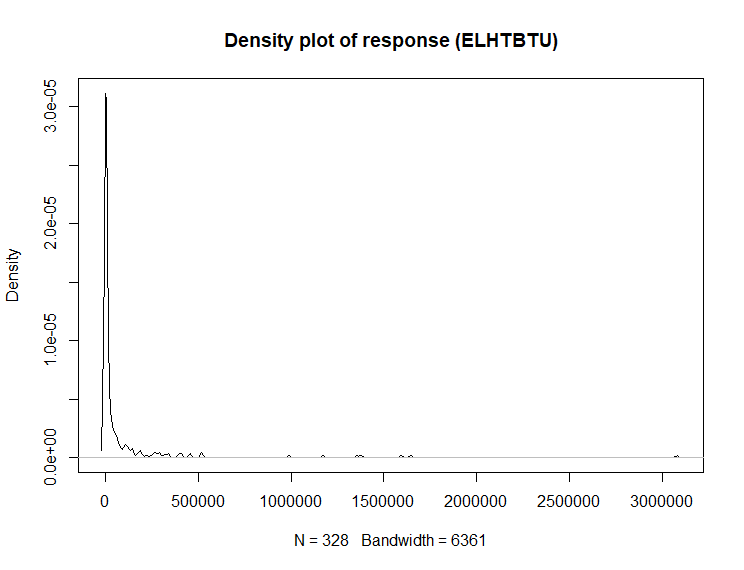
\includegraphics[width=7.6 cm]{densitybefore.png} }}%
    \qquad
    \subfloat{{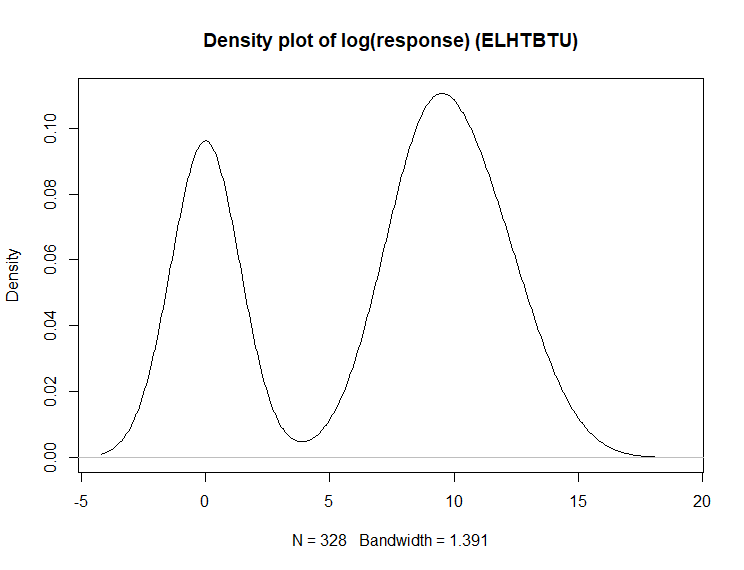
\includegraphics[width=7.6cm]{After.png} }}%
    \label{fig:example}%
    \caption{Before and after log transformation for Response}
\end{figure}

All the predictors and response became normally distributed (however response became bipolar but that's due to lots of zeros in data and won't impact much in our analysis) and we can proceed to modeling part of the problem.
An initial correlation of all the predictors also checked, a brief summary of top predictors correlated with response is as follows:

\begin{table} [H]
\centering 
\begin{tabular}{|c|c|} 
\hline 
Predictor: Categorical & Correlation with Response \\\hline 
Energy used for secondary heating (level - 'NO') & -0.533 \\\
Electricity used for main heating (level - 'NO') & -0.49 \\
Electricity used for secondary heating (level - 'NO') & -0.46 \\
Heat pump heating type: Dual source (level - 'NO') & 0.39 \\
Heat pump heating type: Ground source (level - 'NO') & 0.38\\\hline 
\end{tabular} 
\end{table} 

\begin{table} [H]
\centering 
\begin{tabular}{|c|c|} 
\hline 
Predictor: Numerical & Correlation with Response \\\hline 
Electricity cooling use (thous Btu) & 0.239 \\\
Major fuel cooling use (thous Btu) & 0.237 \\
Electricity water heating use (thous Btu) & 0.227 \\\hline 
\end{tabular} 
\end{table} 

\section{Modeling}
Although, high number of predictors might suggest for a Principal Component Analysis (PCA), it might not be a good idea to use it due to the large number of categorical variables. Even if we convert our categorical variables to dummy variables then also it won't make sense to use PCA because PCA tells us the amount of variance explained by the different predictors and as most of the them are categorical they don't have much variation and hence will not be considered by PCA. This reasoning was also verified by fitting PCA. Instead, following modeling techniques were performed:
\newline

Ridge Regression, LASSO, Random Forest, Gradient Boosting, MARS, BART and Support Vector Machine. Linear regression cannot be done here as the model matrix is a sparse matrix and inverse in not possible.
\newline

First the data was bifurcated into parts i.e. Test and training set in a ratio of 20:80 respectively. Then a 10 fold cross-validation was performed on training data set for tuning parameters for all aforementioned modeling techniques. Finally all models were compared using there performance on test set.

\subsection{Ridge}
As the number of predictors are quite high here, using ridge regression is not a good idea. However, just for the sake of comparison, ridge model was fitted and as expected its performance is not very good with a RMSE value of 3.897 and 3.965 on training and test sets respectively. Lambda vs 'RMSE on training set' plot is shown below for reference.
\begin{figure}[H] 
        \centering 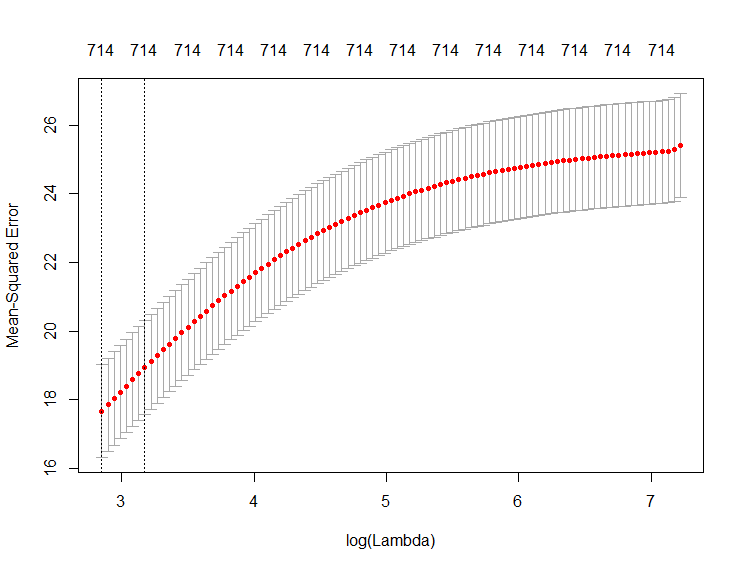
\includegraphics[width=0.7\columnwidth]{ridgelambda.png}
\end{figure}

\subsection{LASSO}
LASSO modeling technique is suitable for such data with huge number of predictors. After tuning lambda value for LASSO using a 10 fold cross validation, lambda providing minimum value of RMSE was chosen i.e. 'lambda.min' = 0.0165. Final RMSE values achieved were 0.655 and 1.154 for testing and training respectively. Model selected from LASSO has a total number of 85 predictors. Lambda vs 'RMSE on training set' plot is shown below for reference.
\begin{figure}[H] 
        \centering 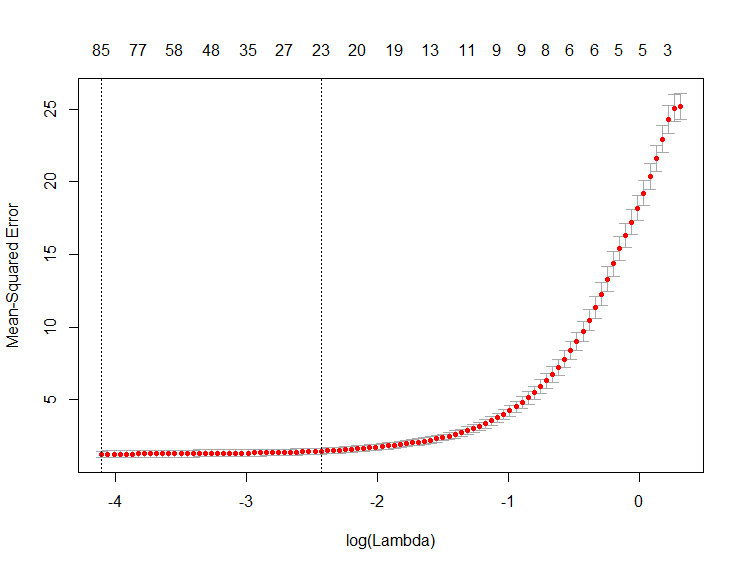
\includegraphics[width=0.7\columnwidth]{LassoLambda.png}
\end{figure}

\subsection{Random Forest}
Parameter tuning for randomForest was done using tuneRF function and optimum value found was mtry = 555. Plot of OOB error vs mtry is shown below for reference. Final RMSE value achieved for training and test sets are 0.996 and 0.52 respectively.
\begin{figure}[H] 
        \centering 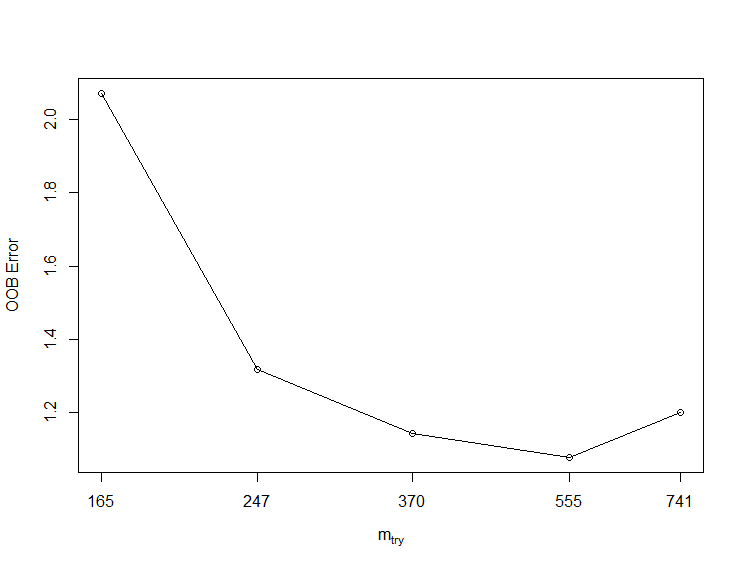
\includegraphics[width=0.7\columnwidth]{mtryselection.png}
\end{figure}

\subsection{MARS}
MARS model was fitted using package earth with a 10 fold cross validation to find optimum number of terms to be taken for a tree. Optimum number of terms included was found 14 for highest R-square (graph shown below). Final RMSE values on training and testing sets are 0.83 and 1.27 respectively.
\begin{figure}[H] 
        \centering 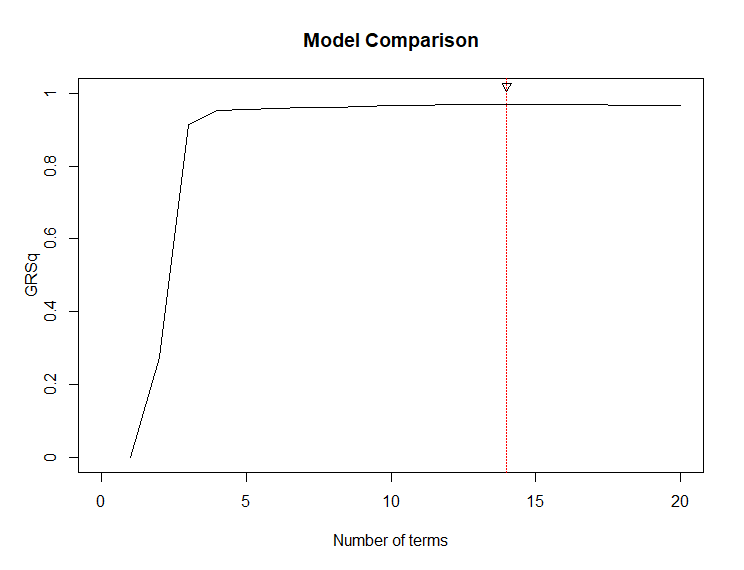
\includegraphics[width=0.7\columnwidth]{Mars.png}
\end{figure}

\subsection{Gradient Boosting}
Gradient boosting model was fitted after tuning requisite parameters which were n.tree = 2000, shrinkage =0.1 and interaction depth = 2 using 10 fold cross validation. Final ntree value was selected by checking model performance on test set, plot showing the same is shown below for reference. Final RMSE values found were 0.36 and 0.99 for training and test set respectively.
\begin{figure}[H] 
        \centering 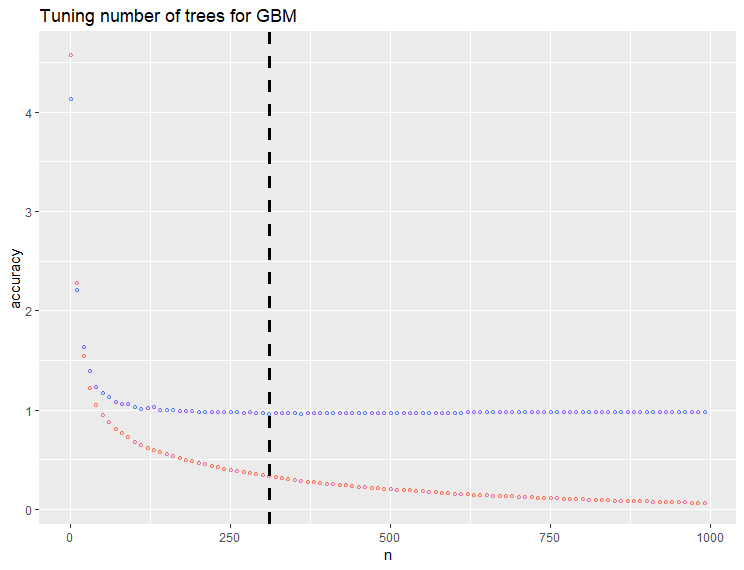
\includegraphics[width=0.65\columnwidth]{gbmntree.png}
\end{figure}

\subsection{BART}
To tune parameters of bartMachine, bartMachineCV() function was used and parameters (nu, q) were tuned. values of parameter m and k were kept fixed at m = 50 trees and k = 2. Final model selected has a RMSE value of 0.458 and 1.111 on training and test set respectively.

\subsection{Support Vector Machine}
SVM parameters were tuned using tune.out function and final RMSE for training and test achieved were 0.99 and 4.7 respectively. Clearly it is not performing well on testing data.
\begin{figure}[H] 
        \centering 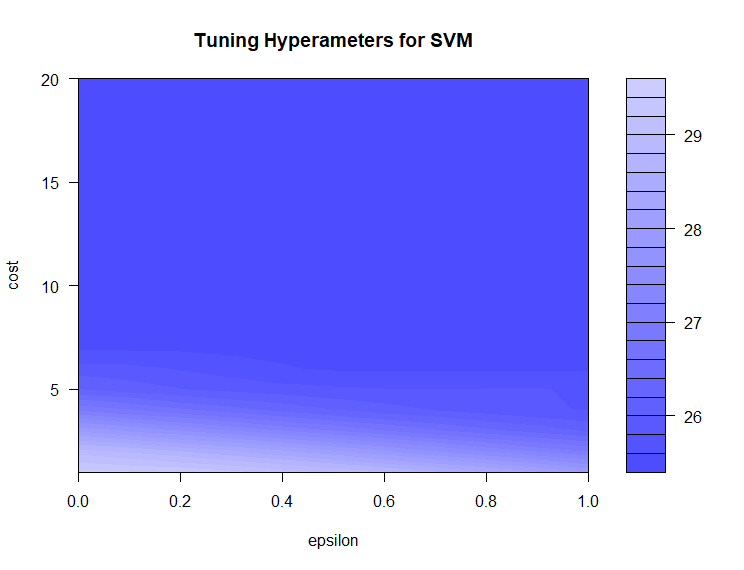
\includegraphics[width=0.62\columnwidth]{svm.png}
\end{figure}

\section{Model Evaluation/Selection}
Final model was selected based on the model performance checked using RMSE values on training and test sets as shown in below graph.
\begin{figure}[H] 
        \centering 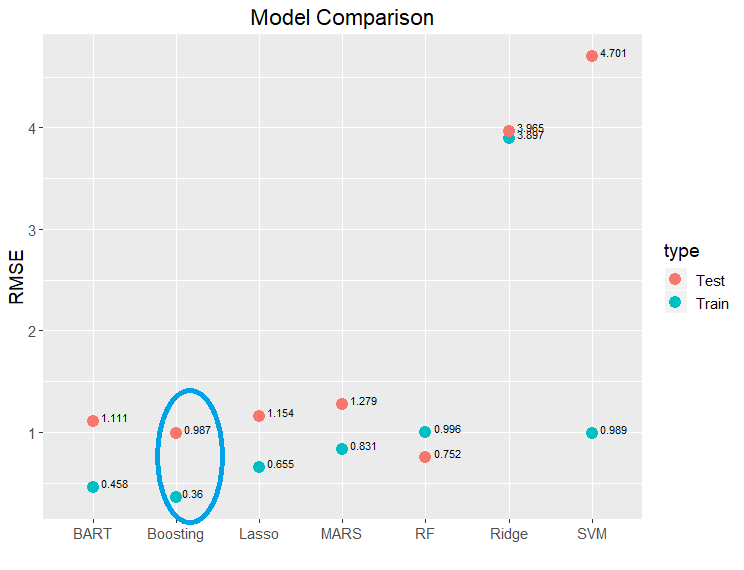
\includegraphics[width=0.75\columnwidth]{comparision.png}
\end{figure}

Best performance is shown by model fitted using gradient boosting technique. Although performance of random forest is also quite good for testing set but its performance on training is not good. Random Forest is performing well on testing set only due to coincidence that the test set chosen during sampling favours this particular model. Final fitted vs actual value graph in shown below.
\begin{figure}[H] 
        \centering 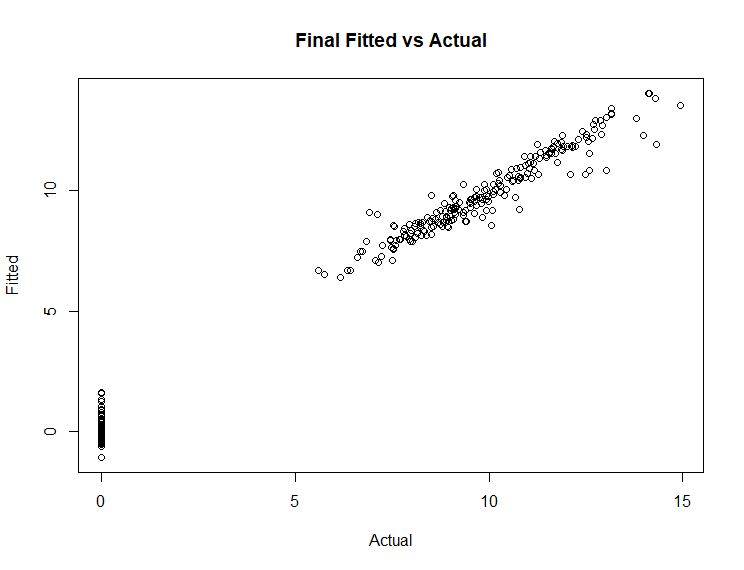
\includegraphics[width=0.75\columnwidth]{finalgraph.png}
\end{figure}

\section{Result Interpretation}
To understand the important predictors we need to further drill down in fitted GBM model. Hence we plotted the variable importance plot for GBM which is shown below. Top 10 predictors impacting the ELHTBTU i.e. Overall electricity used for heating are:

\begin{table} [H]
\centering 
\begin{tabular}{c c c} 
\hline 
Code & Meaning & Correlation \\\hline 
ELHT12 & Electricity not used for main heating & -ve\\\
ELHT22 & Electricity not used for secondary heating & -ve\\
HT22 & Energy not used for secondary heating & -ve\\
ELCLBTU & Electricity cooling use (thous Btu) & +ve\\
MFCLBTU & Major fuel cooling use (thous Btu) & +ve\\
MFLTBTU & Major fuel lighting use (thous Btu) & +ve\\
MFOFBTU & Major fuel office equipment use (thous Btu) & +ve \\
CDD65 & Cooling degree days (base 65) & +ve \\
NOCC & Number of businesses & -ve\\
MFHTBTU & Major fuel heating use (thous Btu) & +ve\\\hline 
\end{tabular} 
\end{table} 

\begin{figure}[H] 
        \centering 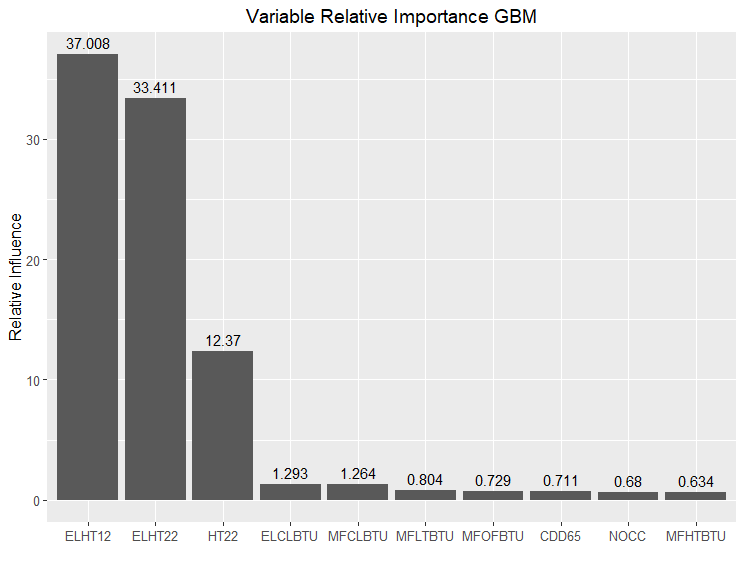
\includegraphics[width=0.75\columnwidth]{gbmvar.png}
\end{figure}

Top 3 predictors are categorical variables signifying following statements:
\begin{itemize}
\item If electricity is not used as main heating, electricity consumption for heating is less.
\item If electricity is not used as secondary heating, electricity consumption for heating is less.
\item If energy is not used for secondary heating, electricity consumption for heating is less.
\end{itemize}

All other top predictors are numerical and their relative influence plots are shown below for further understanding of their impact on response variable. All electricity and fuel consumption data is shown on a logarithmic scale here however if further detailing is required it can be converted to original values exponential function.

\begin{figure}[H]%
    \centering
    \subfloat{{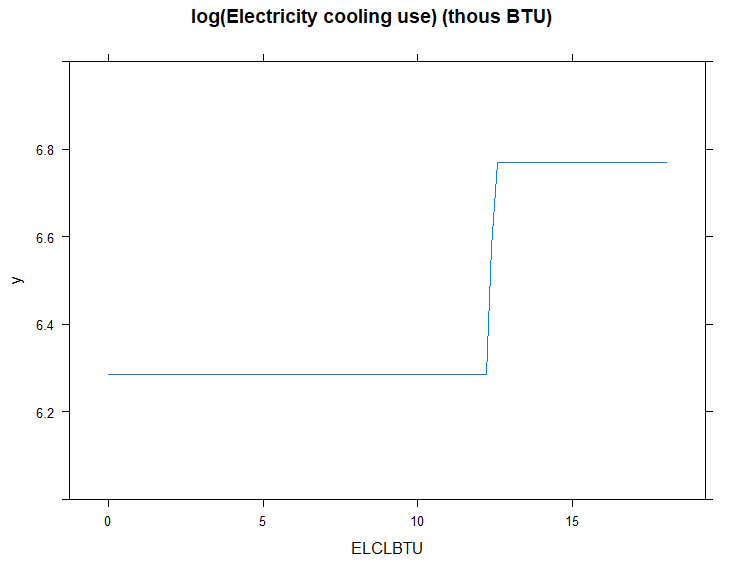
\includegraphics[width= 7.6 cm]{ELCLBTU.png} }}%
    \qquad
    \subfloat{{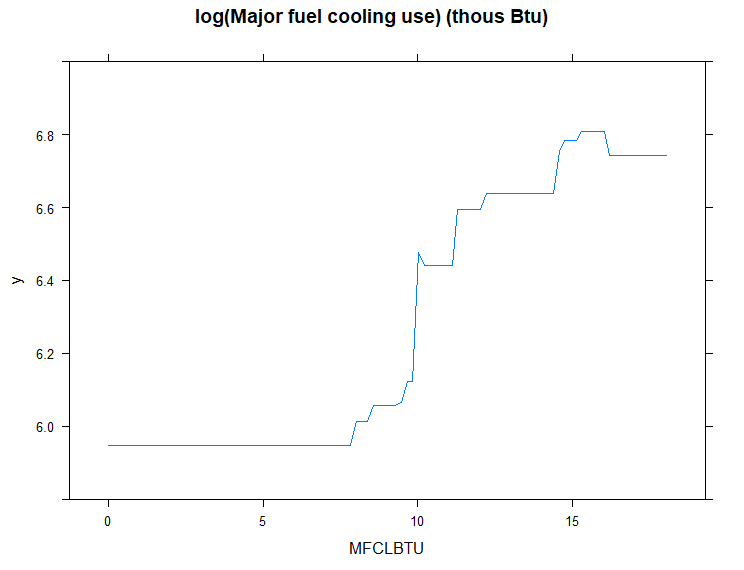
\includegraphics[width= 7.6 cm]{MFCLBTU.png} }}%
    \label{fig:example}%
\end{figure}

From above two plots it can be concluded that if Electricity used for cooling is greater than 260000 BTU or Major fuel used for cooling is greater than 2980 BTU, electricity consumption for heating purpose starts increasing.

\begin{figure}[H]%
    \centering
    \subfloat{{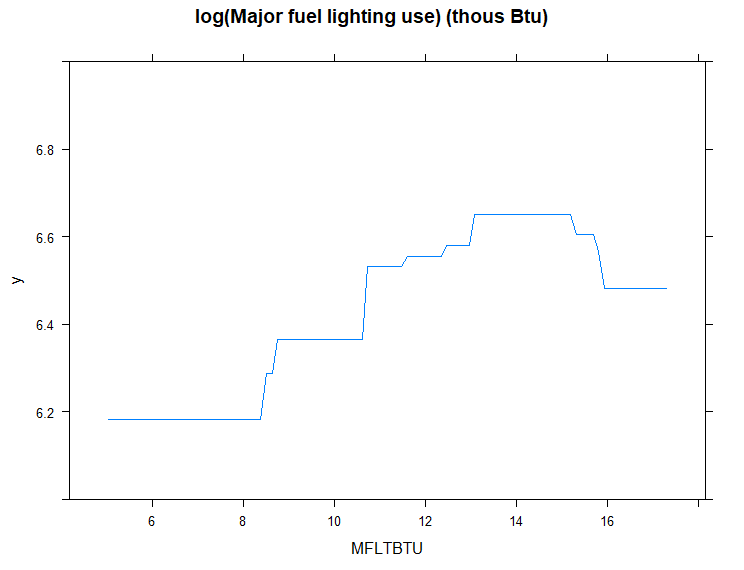
\includegraphics[width=7.6 cm]{MFLTBTU.png} }}%
    \qquad
    \subfloat{{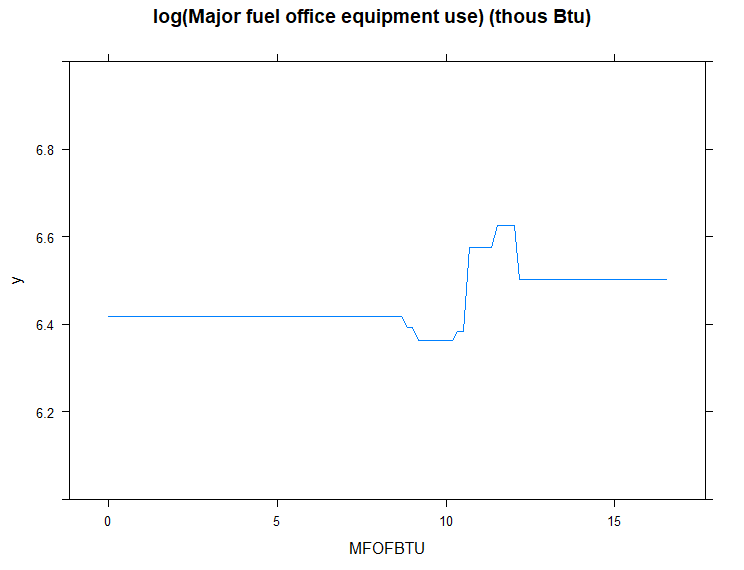
\includegraphics[width=7.6cm]{MFOFBTU.png} }}%
    \label{fig:example}%
\end{figure}

These two plots suggests that if major fuel used for lightening purposes is greater than 250 or major fuel used for office equipment is greater than 1200000 than the electricity used for heating purpose starts increasing. Maybe because more lightening requirement means working at night or cloudy day which signifies colder conditions and hence more electricity usage for heating.

\begin{figure}[H]%
    \centering
    \subfloat{{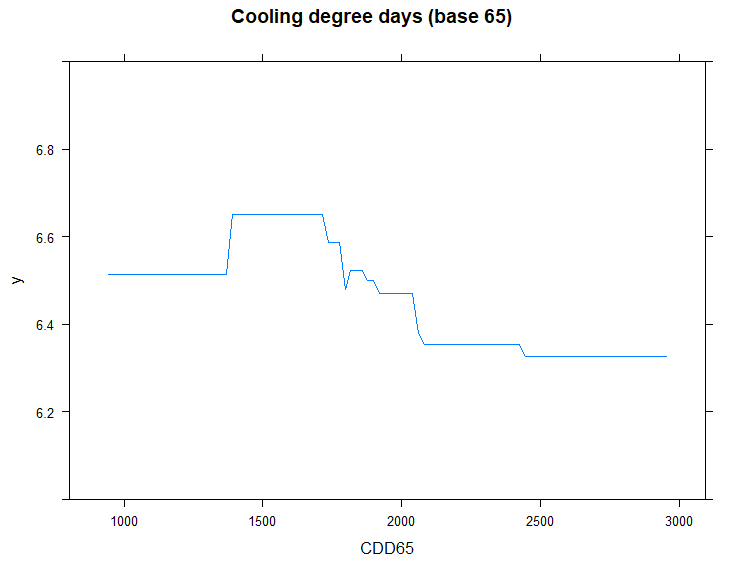
\includegraphics[width=7.6 cm]{CDD65.png} }}%
    \qquad
    \subfloat{{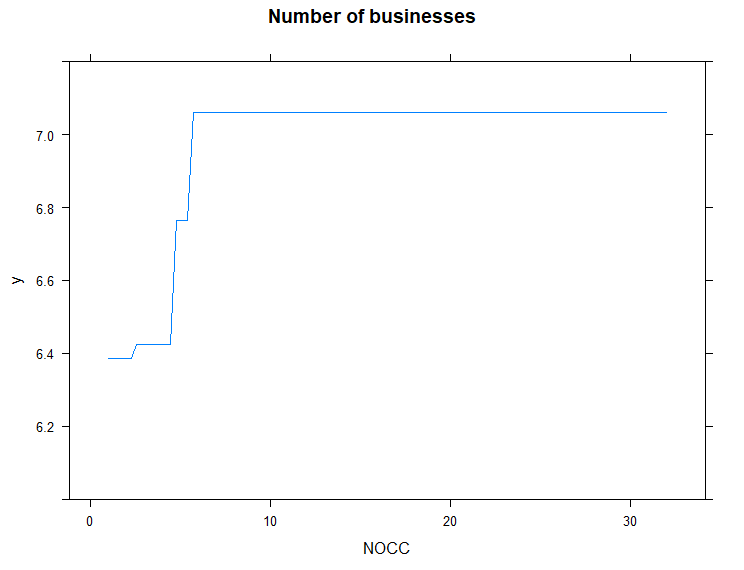
\includegraphics[width=7.6cm]{NOCC.png} }}%
    \label{fig:example}%
\end{figure}

Last two plots suggests that if number of cooling degree days are more i.e. days requiring cooling are more lesser the electricity consumption for heating purposes which makes sense. Also, number of business is more larger is the consumption of electricity for heating purposes.
\section{Overleaf URL}

\url{https://www.overleaf.com/read/ryqcnxkpcwgn}

%++++++++++++++++++++++++++++++++++++++++
% References section will be created automatically 
% with inclusion of "thebibliography" environment
% as it shown below. See text starting with line
% \begin{thebibliography}{99}
% Note: with this approach it is YOUR responsibility to put them in order
% of appearance.
% 




\end{document}

